\usecasebase{Condivisione della prenotazione}
\label{usecase:Condivisione della prenotazione}

\begin{figure}[h]
	\centering
	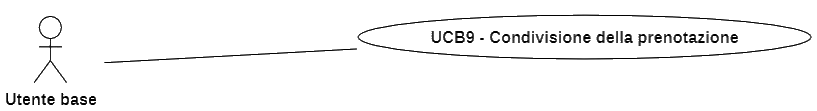
\includegraphics[width=0.8\textwidth]{./uml/UCB9.png} 
	\caption{Condivisione della prenotazione}
	\label{fig:UCB9}
  \end{figure}

\begin{itemize}
	\item \textbf{Attore principale:} Utente base.

	\item \textbf{Precondizioni:}
	\begin{itemize}
		\item L'Utente base ha effettuato l'accesso al Sistema (vedi \autoref{usecase:Effettua accesso}).
		\item L'Utente base sta visualizzando il riepilogo di una prenotazione (vedi \autoref{usecase:Visualizzazione del riepilogo prenotazione}).
	\end{itemize}

	\item \textbf{Postcondizione:}
	      L'Utente base ha copiato il \textit{link} della prenotazione e lo ha condiviso agli altri commensali.

	\item \textbf{Scenario principale:}
	      \begin{enumerate}
		      \item L'Utente base seleziona l'opzione per condividere la prenotazione;
		      \item Il Sistema mostra il \textit{link} della prenotazione;
		      \item L'Utente base copia il \textit{link} della prenotazione;
		      \item L'Utente base invia il \textit{link} agli altri utenti.
	      \end{enumerate}
\end{itemize}
